\newpage
\subsection{Xây dựng hệ thống}

Với yêu cầu của bài toán, ta cần xây dựng hệ thống quản lý văn bằng cho các cơ sở giáo dục, và hệ thống tra cứu thông tin văn bằng cho phía doanh nghiệp (hoặc người có nhu cầu tra cứu).\\

\begin{figure}[ht]
    \centering
    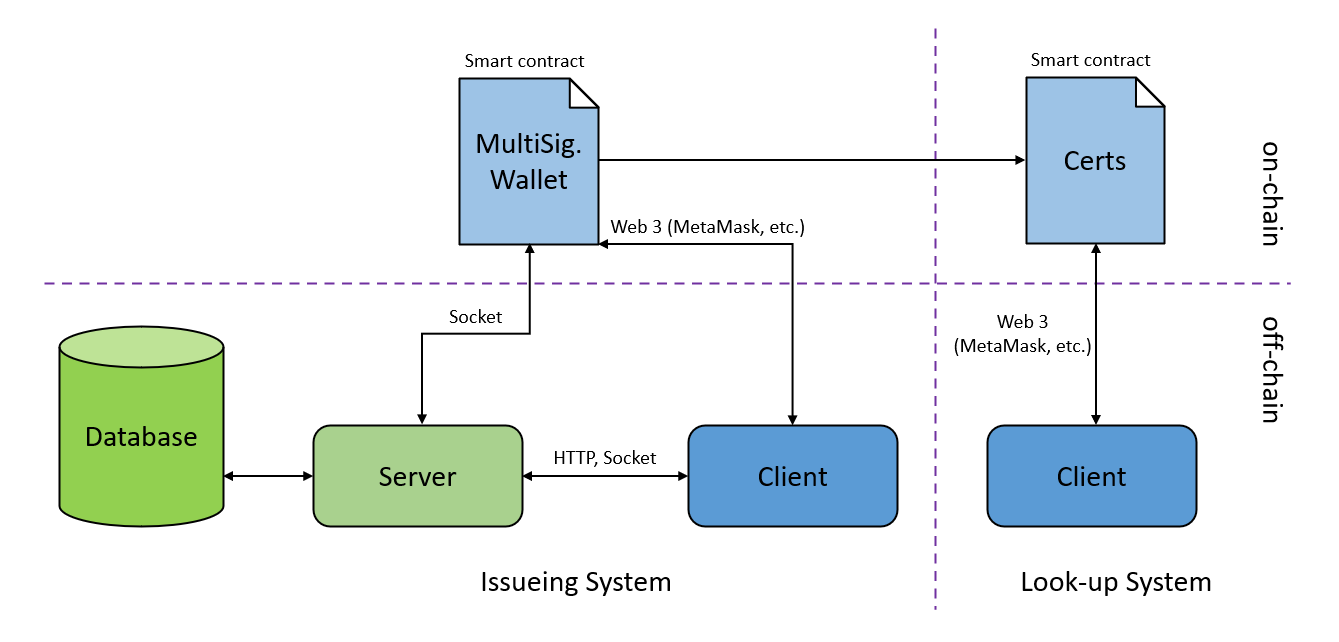
\includegraphics[width=400px]{images/system-overview.png}
\end{figure}

Những hệ thống này sẽ tương tác với các hợp đồng thông minh trên mạng chuỗi khối, bao gồm \textit{Bể văn bằng} (Certs) và \textit{Ví đa chữ ký} (MultiSig. Wallet).

\subsubsection{Bể văn bằng}
\textit{Bể văn bằng} (hay \textit{bể chứng chỉ}) là một hợp đồng thông minh nắm giữ thông tin các văn bằng được lưu trữ trên mạng chuỗi khối.

\subsubsection{Ví đa chữ ký}
\textit{Ví đa chữ ký} là một hợp đồng thông minh với mục đích tăng tính bảo mật cho hệ thống quản lý văn bằng.